Particle physics is the branch of physics that studies the fundamental constituents of matter and the forces governing their interactions.  
The field started as studies in electromagnetism, radiation, and further developed with the discovery of the electron.
What followed was more experiments to search for new particles, new models to describe the results, and new search techniques which demanded more data.
The balance in resources for an experiment bottlenecks how much data can be taken, so steps need to be taken to identify interesting interactions and optimize the storage and processing of this data.
This thesis investigates software performance optimization of the ATLAS experiment at CERN. 
Specifically, ways to modernize and optimize areas of the software framework, Athena, to improve input/output (I/O) performance during derivation production and create new tests that catch when specific core I/O functionality is broken.

\section{LHC and The ATLAS Detector}

\begin{figure}[h]
    \centering
    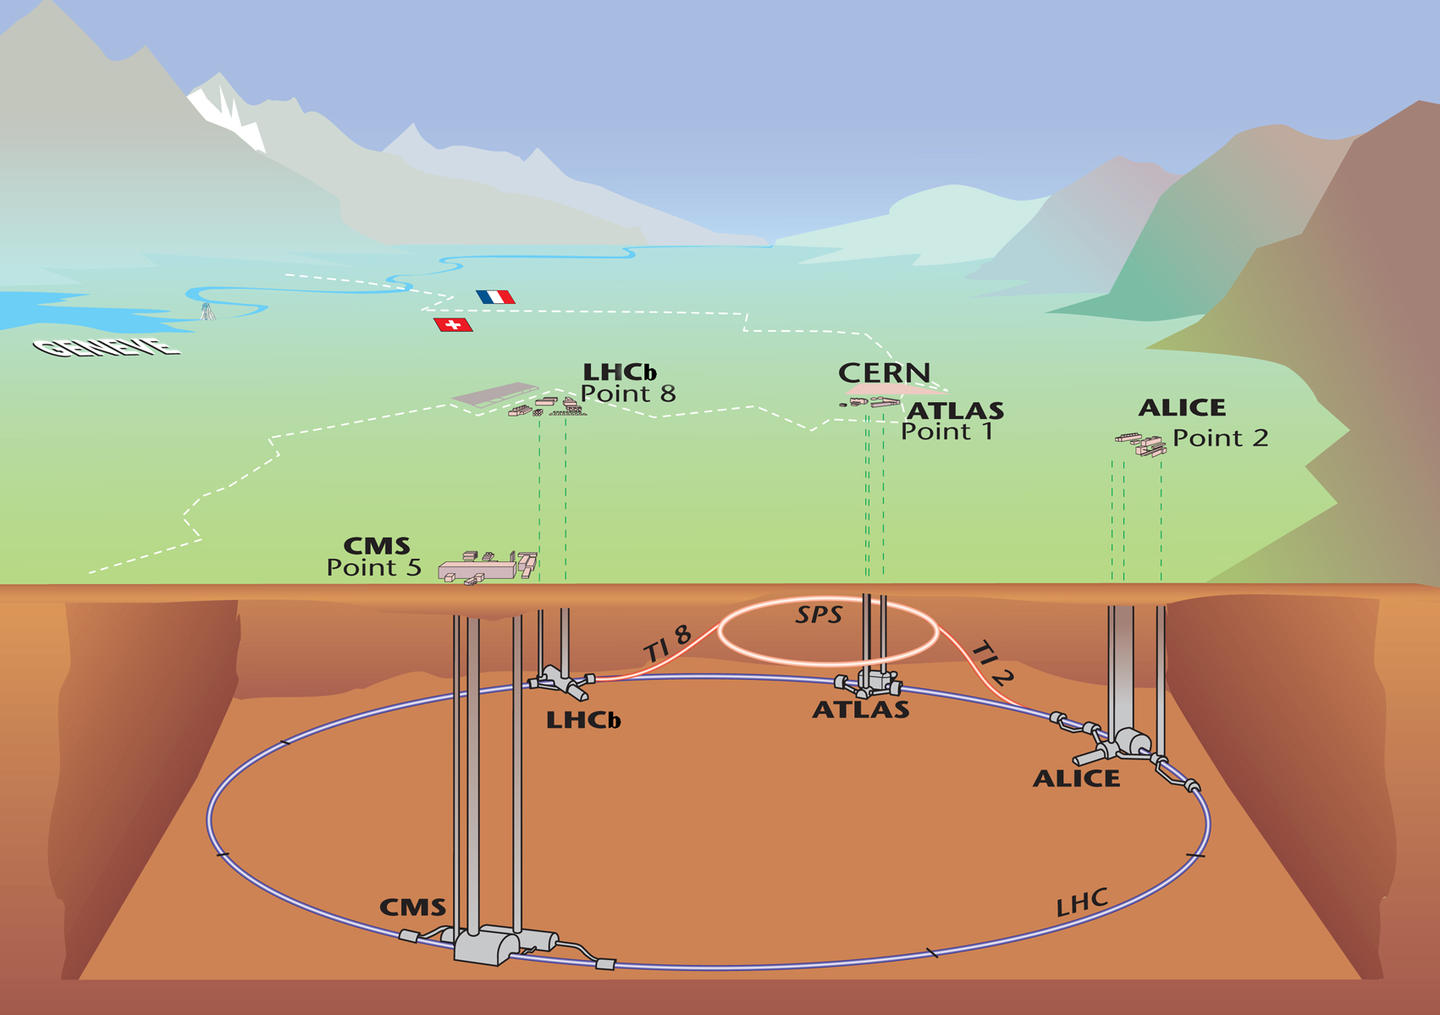
\includegraphics[width=.8\textwidth]{content/img/LHC illustration.jpg}
    \caption{Illustration of the LHC experiment sites on the France-Switzerland border.\cite{LHC_Illustration}}
    \label{fig:intro_LHC_sites}
\end{figure}

The Large Hadron Collider (LHC), shown in Figure \ref{fig:intro_LHC_sites},  is a particle accelerator spanning a 26.7-kilometer ring that crosses between the France-Switzerland border at a depth between 50 and 175 meters underground.\cite{LHC_faq_guide}
The ATLAS experiment, shown in Figure \ref{fig:intro_ATLAS_detector}, is the largest LHC general purpose detector, and the largest detector ever made for particle collision experiments. 
It's 46 meters long, 25 meters high and 25 meters wide.\cite{ATLAS_Fact_Sheet}
The ATLAS detector is comprised of three main sections, the inner detector, calorimeters and the muon detector system. 


\begin{figure}[h]
    \centering
    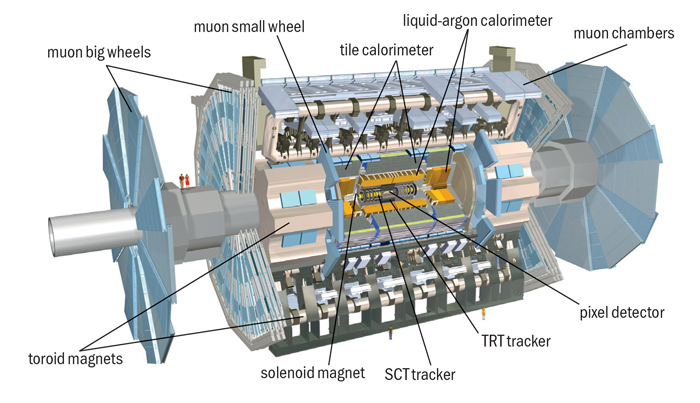
\includegraphics[width=.8\textwidth]{content/img/ATLAS_Detector.jpg}
    \caption{Overview of the ATLAS detectors main components.\cite{ATLAS_Illustration}}
    \label{fig:intro_ATLAS_detector}
\end{figure}


The inner detector measures the direction, momentum and charge of electrically charged particles.
Its main function is to measure the track of the charged particles without destroying the particle itself.
The first point of contact for particles emerging from $pp$-collisions from the center of the ATLAS detector is the pixel detector.\cite{PixelDetector_2008}
It has over 92 million pixels and is radiation hard to aid in particle track and vertex reconstruction.
When charged particles pass through a pixel sensor, it ionizes the one-sided doped-silicon wafer to produce an excited electron will then occupy the conduction band of the semiconductor producing an electron-hole pair, leaving the valence band empty.\cite{KnollRadDetection}
This hole in the valence band together with the excited electron in the conduction band is called an electron-hole pair.
The electron-hole pair is in the presence of an electric field, which will induce drifting of the electron-hole pair, drifting that will generate the electric current to be measured.

Surrounding the pixel detector is the SemiConductor Tracker (SCT), which uses 4,088 modules of 6 million implanted silicon readout strips.\cite{ABDESSELAM2006642}
Both the pixel detector and SCT measure the path particles take, called tracks.
While the pixel detector has measurement precision up to $10 \mu m$, the SCT has precision up to $25\mu m$. 

The final layer of the inner detector is the transition radiation tracker (TRT). 
The TRT is made of a collection of tubes made with many layers of different materials with varying indices of refraction.
The TRT's straw walls are made of two $35\mu m$ layers comprised of $6\mu m$ carbon-polymide, $0.20 \mu m$ aluminum, and a $25\mu m$ Kapton film reflected back.\cite{TRT_2008}
The straws are filled with a gas mixture of $70\% \text{Xe} + 27\% \text{CO}_2 + 3\% \text{O}_2$. 
Its measurement precision is around $170 \mu m$. 
Particles with relativistic velocities have higher Lorentz $\gamma$-factors (see Equation \eqref{lorentzGamma}). 
The TRT uses varying materials to discriminate between heavier particles, which have low $\gamma$ and radiate less, and lighter particles, which have higher $\gamma$ and radiate more.\cite{Mindur:2139567}
\begin{equation}\label{lorentzGamma}
    \gamma = \frac{1}{\sqrt{1 - \frac{v^2}{c^2}}}
\end{equation}

There are two main calorimeters for ATLAS, the Liquid Argon (LAr) calorimeter and the Tile Hadronic calorimeter.
The LAr calorimeter surrounds the inner detector and measures the energy deposits of electrons, photons and hadrons (quark bound states, such as baryons $qqq$ and mesons $q\bar{q}$). 
It layers various metals to intercept the incoming particles to produce a shower of lower energy particles. 
The lower energy particles then ionize the liquid argon that fill the barrier in between the metal layers to produce a current that can be read out.
The Tile calorimeter surrounds the LAr calorimeter and is the largest part of the ATLAS detector weighing in around 2900 tons. 
Particles then traverse through the layers of steel and plastic scintillating tiles. 
When a particle hits the steel, a cascade of secondary particles is generated, and the plastic scintillators will produce photons whose current can be measured.

\section{ATLAS Trigger and Data Acquisition (DAQ)}

The LHC produces $pp$-collisions at a rate of 40 MHz, each collision is an ``event". 
% What is the ATLAS Trigger System
The ATLAS Trigger system is responsible for quickly deciding what events are interesting for physics analysis.
The Trigger system is divided into the first- and second-level triggers and when a particle activates a trigger, the trigger makes a decision to tell the Data Acquistion System (DAQ) to save the data produced by the detector. 
The first-level trigger is a hardware trigger that decides, within $2.5 \mu s$ after the event, if it's a good event to put into a storage buffer for the second-level trigger.
The second-level trigger is a software trigger that decides within $200 \mu s$ and uses around 40,000 CPU-cores and analyses the event to decide if it is worth keeping. 
The second-level trigger selects about 1000 events per second to keep and store long-term.\cite{Trigger-DAQ}
The data taken by this Trigger/DAQ system is raw and not yet in a state that is ready for analysis, but it is ready for the reconstruction stage. 

% How is this relevant to the thesis?
The amount of data taken at ATLAS is substantial.
ATLAS sees more than 3.2 PB of raw data each year, each individual event being around 1.6 MB.\cite{ATLAS_Fact_Sheet} 
All of the data produced by LHC experiments, especially ATLAS, has to be sent to the LHC Computing Grid (LCG). 
The increase in data means more resources from the Grid will be needed, so optimization is an essential part of ensuring scalability of the data able to be taken in by the experiment.
Reconstructed AOD are then processed through derivation jobs that reduced AODs from  $\mathcal{O}(1)$ MB per event to $\mathcal{O}(10)$ kB per event, creating Derived AOD (DAOD). 

\section{HL-LHC and Future Needs in Computation}
The High-Luminosity LHC (HL-LHC) is the upgrade to LHC that anticipates more events and more data taken than ever before.
% How does high luminosity affect the number of collisions? 
The goal is to reach a luminosity of $350 fb^{-1}$, which is forecasted to be reached gradually by around 2040.\cite{HL-LHC_Tech_design}
The HL-LHC era is projected to demand anywhere from 6-10 times data stored per year, so any attempt to save on disk storage will help.\cite{ATLAS_HL-LHC_projections}

One area of research to account for this flood of new data is in the development of the ROOT N-Tuple (RNTuple) I/O subsystem, which is a new storage format for high-energy physics data seeking to replace ROOT TTree. 
The RNTuple is a columnar-based storage format that is optimized for data storage and processing.
It's been shown to outperform TTree I/O subsystem and other storage formats in file size (by about 15\%), throughput, and compression, but still has more development before full implementation into the analysis pipeline.\cite{RNTuple_Lopez-Gomez_2023}\cite{RNTuple_Blomer}
Additionally, there's a push to utilize GPUs and other accelerators in conjunction with CPUs to process track reconstruction and AOD derivation.
Also being developed are software framework updates, such as AthenaMT, to make the single-threaded CPU programs multi-thread ready.\cite{AthenaMT_Leggett_2017}

